\chapter{Introducción}

El \textit{Aprendizaje por Refuerzo} (\textit{Reinforcement Learning}, RL) se ha consolidado como una de las ramas más activas y prometedoras del aprendizaje automático. A diferencia del aprendizaje supervisado, en el que el modelo aprende a partir de ejemplos etiquetados, el RL se fundamenta en la interacción continua de un agente con un entorno, buscando maximizar una recompensa acumulada. Este paradigma ha permitido resolver problemas complejos de toma de decisiones secuenciales en campos tan diversos como la robótica, los videojuegos, la gestión de recursos o la conducción autónoma.

En los últimos años, la combinación del RL con redes neuronales profundas —conocida como \textit{Deep Reinforcement Learning} (DRL)— ha supuesto un gran avance, al permitir que los agentes aprendan directamente a partir de observaciones de alta dimensión. Algoritmos como \textit{Deep Q-Network} (DQN) o \textit{Proximal Policy Optimization} (PPO) han demostrado su eficacia en entornos complejos como Atari o MuJoCo, donde el espacio de estados y de acciones puede ser extremadamente amplio.

Sin embargo, el rendimiento de un agente no depende únicamente del algoritmo de aprendizaje empleado, sino también de la representación del estado con la que percibe el entorno. En otras palabras, la complejidad de la observación influye directamente en la capacidad del agente para generalizar, explorar y aprender políticas efectivas. Representaciones demasiado simples pueden limitar el aprendizaje al ocultar información relevante, mientras que representaciones demasiado complejas pueden ralentizar la convergencia y requerir una mayor capacidad de red o una exploración más prolongada.

En este Trabajo Fin de Máster se analiza precisamente cómo afecta la complejidad del estado observado al rendimiento del agente en un entorno controlado. Para ello, se ha desarrollado un entorno propio denominado \textit{SimplePacmanEnv}, inspirado en el clásico juego \textit{Pac-Man}, pero adaptado para experimentos de RL. Este entorno, implementado con \textit{Gymnasium} y \textit{Stable-Baselines3}, permite configurar diferentes niveles de complejidad en la observación —desde representaciones mínimas (solo posiciones del jugador y el fantasma) hasta observaciones enriquecidas con información global sobre las monedas o incluso representaciones tipo imagen—, manteniendo constantes la dinámica del entorno y la estructura de recompensas.

Sobre esta base se han entrenado y evaluado tres algoritmos representativos de distintas familias del RL profundo: \textit{Advantage Actor-Critic} (A2C), \textit{Proximal Policy Optimization} (PPO) y \textit{Deep Q-Network} (DQN). El objetivo es cuantificar cómo evoluciona el aprendizaje y el rendimiento final de cada agente en función de la información proporcionada por el entorno, y determinar si existe una relación clara entre la complejidad de la representación del estado y la eficiencia del aprendizaje.

Además, el proyecto incorpora herramientas complementarias como \textit{TensorBoard} para la monitorización en tiempo real del entrenamiento, y el uso de \textit{EvalCallback} para realizar evaluaciones periódicas y registrar automáticamente el mejor modelo alcanzado. Estos mecanismos no solo facilitan el análisis experimental, sino que aportan rigor y reproducibilidad a los resultados obtenidos.

En conjunto, este trabajo busca aportar una visión práctica y experimental sobre la influencia de la observación en entornos de aprendizaje por refuerzo, conectando los fundamentos teóricos con un estudio aplicado y reproducible, y poniendo de manifiesto la importancia del diseño de los estados en la efectividad de los algoritmos de RL.

\begin{figure}[h]
\centering
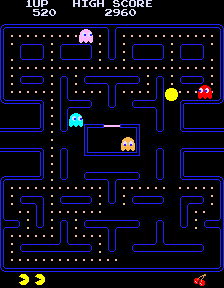
\includegraphics[width=0.5\textwidth]{./figs/image1.png}
\caption{Imagen del juego original de Pac-man de 1980}
\label{fig:screenshot_pacman}
\end{figure}

\section{Contexto y motivación}

\subsection{Justificación e interés}
El estudio de la relación entre la complejidad del estado y el rendimiento del agente resulta relevante tanto desde el punto de vista teórico como práctico:

\begin{itemize}
    \item Permite entender la eficiencia y capacidad de generalización de distintos algoritmos (A2C, PPO, DQN) en entornos de distinta dimensionalidad.
    \item Aporta evidencia empírica sobre el compromiso entre simplicidad del modelo y capacidad de representación, tema central en el diseño de entornos y arquitecturas RL.
    \item Facilita la comparación controlada entre configuraciones de observación, aislando el impacto del estado sin alterar dinámicas, recompensas ni mecánicas de juego.
    \item Además, el uso de un entorno propio y reproducible contribuye al valor educativo e investigativo, permitiendo futuras extensiones y análisis.
\end{itemize}

\subsection{Motivación personal}

Mi motivación para realizar este proyecto es principalmente educativa e investigativa.
Busco profundizar en el campo del Aprendizaje por Refuerzo, comprendiendo de forma práctica cómo los agentes aprenden a través de la interacción con su entorno y cómo la cantidad de información observada afecta dicho proceso.

El trabajo ha supuesto un ejercicio de integración de conocimientos adquiridos durante el Máster (aprendizaje automático, programación en Python, redes neuronales, y metodologías experimentales) con el objetivo de desarrollar una visión más completa y aplicada del RL.
En última instancia, la meta ha sido explorar, aprender y comprender los fundamentos de la toma de decisiones secuenciales bajo incertidumbre.

\section{Objetivos}

\subsection{Objetivo principal}

Evaluar cómo el nivel de complejidad del espacio de observación afecta el rendimiento de distintos algoritmos de Aprendizaje por Refuerzo, manteniendo constantes el entorno, las recompensas y la dinámica del juego.

\subsection{Objetivos específicos}

\begin{enumerate}
    \item Diseñar e implementar un entorno controlado y parametrizable (basado en Pac-Man) que permita modificar el tipo de observación percibida por el agente.
    \item Entrenar y comparar varios algoritmos de RL (A2C, PPO, DQN) bajo distintos modos de observación.
    \item Analizar métricas de rendimiento (recompensa media, estabilidad, convergencia, tiempo de entrenamiento).
    \item Evaluar la relación entre dimensionalidad del estado y eficiencia del aprendizaje.
    \item Documentar la metodología y resultados, destacando las implicaciones para futuros desarrollos o estudios.
\end{enumerate}

\section{Sostenibilidad, diversidad y desafíos ético/sociales}

A continuación se valoran los posibles impactos en materia de sostenibilidad, ética y diversidad.

\paragraph{Sostenibilidad.}
El trabajo se ha realizado íntegramente en un entorno digital y no requiere recursos materiales adicionales, por lo que su impacto medioambiental directo es muy reducido. El único consumo relevante proviene del uso de recursos computacionales durante el entrenamiento de los agentes. Se ha procurado minimizar este impacto mediante el uso de modelos ligeros y tiempos de entrenamiento moderados, evitando configuraciones innecesariamente costosas. Desde una perspectiva positiva, la metodología promueve la eficiencia en la experimentación mediante la reutilización de entornos y scripts reproducibles, contribuyendo así a un uso más sostenible de los recursos de investigación. El proyecto no se ve afectado por ninguna normativa específica en materia medioambiental ni tiene relación directa con los Objetivos de Desarrollo Sostenible (ODS), más allá de fomentar el desarrollo de tecnologías digitales eficientes y abiertas.

\paragraph{Comportamiento ético y responsabilidad social.}
El proyecto no involucra datos personales, información sensible ni toma de decisiones sobre personas o colectivos. Su propósito es exclusivamente académico y experimental. Se han seguido principios de transparencia y reproducibilidad, haciendo uso de bibliotecas abiertas como \textit{Stable-Baselines3} y \textit{Gymnasium}, lo que garantiza la trazabilidad del código y los resultados. En este sentido, el trabajo se alinea con los principios deontológicos de la ingeniería informática, promoviendo la investigación responsable y el acceso abierto al conocimiento. No se identifican impactos negativos sobre el empleo ni sobre aspectos legales o de seguridad.

\paragraph{Diversidad, género y derechos humanos.}
El contenido técnico del trabajo no tiene incidencia directa en cuestiones de género, diversidad o derechos humanos. Sin embargo, se reconoce la importancia de la diversidad en la investigación en inteligencia artificial y el compromiso con un lenguaje inclusivo y accesible en la documentación y la memoria del proyecto. Asimismo, el entorno desarrollado puede emplearse como herramienta docente o de experimentación, favoreciendo la accesibilidad y la igualdad de oportunidades en la formación en técnicas de aprendizaje por refuerzo.

En conjunto, el proyecto presenta un impacto ético, social y medioambiental neutro o ligeramente positivo, destacando por su orientación a la investigación abierta, la eficiencia computacional y el cumplimiento de buenas prácticas profesionales en el ámbito de la inteligencia artificial.


\section{Enfoque y metodología}

El presente trabajo adopta un enfoque experimental y comparativo orientado a analizar la influencia de la complejidad del estado sobre el rendimiento de los algoritmos de Aprendizaje por Refuerzo (RL).

\subsection{Estrategias consideradas}

Durante la fase inicial del proyecto se evaluaron tres posibles enfoques:

\begin{enumerate}
	\item \textbf{Uso de entornos estándar (Gym / Atari):}
Permitiría aprovechar entornos consolidados como CartPole o Breakout. Sin embargo, estos no ofrecen un control granular sobre la estructura del estado, lo que impide aislar experimentalmente el efecto de la observación.
	\item \textbf{Simulación matemática abstracta (MDP sintético):}
Un enfoque más teórico, usando representaciones vectoriales arbitrarias para estudiar el tamaño del espacio de estado. Aunque más simple de implementar, carece de un contexto visual y de dinámica tangible que facilite la interpretación y comparación intuitiva de los resultados.
	\item \textbf{Diseño de un entorno personalizado (Pacman simplificado):}
Este enfoque combina realismo y control. Permite modificar el nivel de información observable manteniendo constantes las reglas y recompensas.
Además, el dominio es familiar y visualmente interpretable, lo que facilita tanto la depuración como la comunicación de los resultados.
\end{enumerate}

\subsection{Estrategia seleccionada}

Se eligió la \textbf{tercera estrategia}, basada en el desarrollo de un entorno propio —SimplePacmanEnv— compatible con Gymnasium y Stable-Baselines3.
Esta elección resulta la más adecuada por las siguientes razones:

\begin{itemize}
	\item Permite \textbf{aislar experimentalmente} la variable de interés (la complejidad del estado), manteniendo el resto de factores constantes.
	\item Facilita la \textbf{comparación justa} entre distintos algoritmos de RL bajo las mismas condiciones.
	\item Favorece la \textbf{reproducibilidad y extensibilidad} del experimento (se pueden añadir observaciones o cambiar reglas sin alterar la estructura general).
	\item Proporciona una \textbf{base educativa sólida}, al exigir una comprensión integral del pipeline de RL: diseño de entorno, configuración del agente y análisis de resultados.
\end{itemize}